\documentclass[a4paper]{article}
\usepackage[14pt]{extsizes} 
\usepackage[T2A]{fontenc}
\usepackage[utf8]{inputenc}
\usepackage{natbib}
\usepackage{graphicx}
\usepackage{amsmath}
\usepackage[english]{babel}
\usepackage{fontspec}
\usepackage{amsmath,amsfonts,amssymb,amsthm,mathtools,mathrsfs}
\usepackage{icomma}
\usepackage{fullpage}
\usepackage{ulem}
\usepackage{eufrak}
\usepackage{setspace}
\usepackage{listings}
\usepackage{indentfirst}
\usepackage[left=2cm,right=1.5cm,top=2cm,bottom=2cm]{geometry}
\usepackage{xcolor}
\usepackage{float}
\usepackage{csquotes}

\setmainfont[Ligatures={TeX,Historic}]{Times New Roman}
\setlength{\parindent}{5ex}
\setlength{\parskip}{1em}
\renewcommand{\baselinestretch}{1}

\graphicspath{{images/}}

\definecolor{buzzlightyear}{HTML}{8757A5}
\definecolor{grass}{HTML}{738D06}
\definecolor{literal}{HTML}{F18A2B}
\definecolor{commentcolor}{HTML}{8E908B}

\lstdefinestyle{habrstyle}{
    backgroundcolor=\color{white},   
    commentstyle=\color{commentcolor},
    keywordstyle=\bfseries\color{buzzlightyear},
    numberstyle=\tiny\color{commentcolor},
    stringstyle=\color{grass},
    basicstyle=\ttfamily\footnotesize,
    breakatwhitespace=false,         
    breaklines=true,                 
    captionpos=b,                    
    keepspaces=true,                 
    numbers=left,                    
    numbersep=5pt,                  
    showspaces=false,                
    showstringspaces=false,
    showtabs=false,                  
    tabsize=4
}

\lstset{style=habrstyle}

\begin{document}

    % FIRST PAGE
    \begin{center}
        \begin{center}
        \hfill \break
        \normalsize{Санкт-Петербургский государственный политехнический}\\
        \normalsize{университет Петра Великого}\\
        \hfill \break
        \normalsize{\textbf{Высшая школа интеллектуальных систем и}}\\ 
        \normalsize{\textbf{суперкомпьютерных технологий}}\\ 
        \hfill \break
        \hfill \break
        \hfill \break
        \normalsize{Лабораторная работа}\\
        \hfill \break
        \hfill \break
        \normalsize{\LARGE Апериодические сигналы}\\
        \end{center}
        \hfill \break
        \hfill \break
        \hfill \break
        \hfill \break
        \hfill \break
        \hfill \break
        \hfill \break
        \hfill \break
        \hfill \break
        \hfill \break
        \begin{flushright}
            \normalsize{Работу выполнил студент}\\
            \normalsize{3-го курса, группа 3530901/80201}\\
            \normalsize{Сахибгареев Рамис Ринатович}\\
            \hfill \break
            \normalsize{Преподаватель:}\\
            \normalsize{Богач Наталья Владимировна}\\
        \end{flushright}
        \hfill \break
        \hfill \break
        \hfill \break
        \hfill \break
        \begin{center} Санкт-Петербург 2021 \end{center}
        \thispagestyle{empty}
    \end{center}
    % FIRST PAGE [END]
    
    \newpage
        \tableofcontents
    
    \newpage
         \listoffigures
    
    \newpage
         \lstlistoflistings   
     
    % START START START START START
    \newpage
        \section{Part 1: Examples execution}
        
        In this part we need to execute every part of "chap3" file. By executing it we can take a brief look on the chirp signals and spectrograms and windows.
        
        After executing every input in "chap3" file no problems was found. Different windows was tested, they close to each other, but has different impact on the signal. (Listing \ref{lst:part1_1}, Figure \ref{fig:work_check}).
        
        \begin{lstlisting}[language=Python,caption=Windows computation,label={lst:part1_1}]
    wave = signal.make_wave(duration)
    wave.window(np.bartlett(len(wave)))
    spectrum = wave.make_spectrum()
    spectrum.plot(high=880, color='red')
    decorate(xlabel='Frequency (Hz)')
    
    wave = signal.make_wave(duration)
    wave.window(np.blackman(len(wave)))
    spectrum = wave.make_spectrum()
    spectrum.plot( high=880, color ='green')
    decorate(xlabel ='Frequency (Hz)')
    
    wave = signal.make_wave(duration)
    wave.window(np.kaiser(len(wave), 10))
    spectrum = wave.make_spectrum()
    spectrum.plot(high =880, color ='blue')
    decorate(xlabel ='Frequency (Hz)')
    
    wave = signal.make_wave(duration)
    wave.window(np.hanning(len(wave)))
    spectrum = wave.make_spectrum()
    spectrum.plot(high =880, color ='#FF00FF')
    decorate(xlabel ='Frequency (Hz)')
        \end{lstlisting}
        
        \begin{figure}[h]
            \centering
            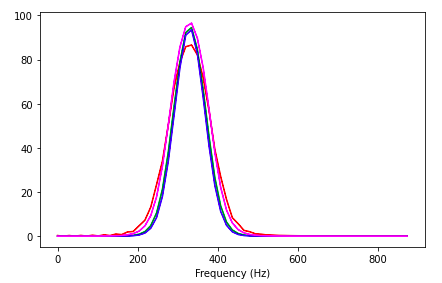
\includegraphics[width=\textwidth]{img/yotsunomado.png}
            \caption{Different windows}
            \label{fig:work_check}
        \end{figure}
    
    \newpage
        \section{Part 2: SawtoothChirp}

        In this part we need to create a \texttt{SawtoothChirp} class, that extends the \texttt{Chirp} class and provides an \texttt{evaluate} function. After it's done we can create its spectrogram.
        
        Let's declare a class (Listing \ref{lst:sawtooth_def})
            
        \begin{lstlisting}[language=Python,caption={Sawtooth class definition},label={lst:sawtooth_def}]
    from thinkdsp import *
    import numpy as np
    
    class SawtoothChirp(Chirp):
        def evaluate(self, ts):
            # freq change
            freqs = np.linspace(self.start, self.end, len(ts) - 1)
            # steps
            dts = np.diff(ts)
            dphis = PI2 * freqs * dts
            phases = np.cumsum(dphis)
            # apply default sawtooth code
            cycles = phases / PI2
            frac, _ = np.modf(cycles)
            ys = normalize(unbias(frac), self.amp)
            return ys
        \end{lstlisting}
        
        
        
        Next, we can check is our class works correctly (Listing \ref{lst:sawtooth_check}, Figure \ref{fig:sawtooth_wave_plot}).
            
        \begin{lstlisting}[language=Python,caption=Sawtooth wave plot code,label={lst:sawtooth_check}]
    sawtooth = SawtoothSignal()
    sawtooth_wave = sawtooth.make_wave(sawtooth.period * 3, framerate=40000)
    sawtooth_wave.plot()
    decorate(xlabel='Time (s)')
        \end{lstlisting}

        \begin{figure}[H]
          \centering
          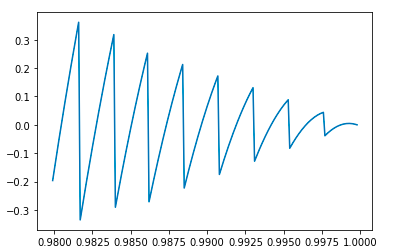
\includegraphics[width=\textwidth]{img/saw_c.png}
          \caption{Sawtooth's wave's plot}
          \label{fig:sawtooth_wave_plot}
        \end{figure}
            
        Next, spectrogram for created signal was created (Listing \ref{lst:sawtooth_spec}, Figure \ref{fig:sawtooth_spec}).
            
        \begin{lstlisting}[language=Python,caption=Sawtooth's spectrum computation,label={lst:sawtooth_spec}]
    s = wave.make_spectrogram(256)
    s.plot()
    decorate(xlabel='Time (s)', ylabel='Frequency (Hz)')
        \end{lstlisting}
        
        \begin{figure}[H]
          \centering
          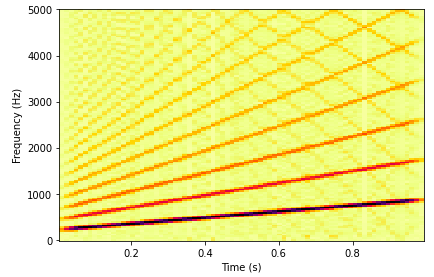
\includegraphics[width=\textwidth]{img/sew_s.png}
          \caption{Sawtooth's spectrogram}
          \label{fig:sawtooth_spec}
        \end{figure}
        
    \newpage
        \section{Part 3: Changing Sawtooth}
            
        In this part we need to explore the aliasing effect on the Sawtooth chirp. 
        
        To reproduce this effect let's create a sawtooth chirp of frequency 2500 Hz to 3000 Hz and framerate of 20000 Hz (Listing \ref{lst:als_sqr}, Figure \ref{fig:als_sqr}). We can clearly see wide main frequency components and a lot of noise. It happens because main components and aliase components are "drifting" to the higher frequency with the time, and spectrum shows overall spectrum of the sound. We can make spectrogram clearer, by increasing the wave's framerate (Figure \ref{fig:als_clr}).
        
        
            
        \begin{lstlisting}[language=Python,caption=Waves creation,label={lst:als_sqr}]
    wave = SquareSignal(1100).make_wave(duration=9.6, framerate=10000)
    wave_clear = SquareSignal(1100).make_wave(duration=1, framerate=96000)
    wave.make_spectrum().plot(color='red')
    wave_clear.make_spectrum().plot(color='blue')
        \end{lstlisting}
            
        \begin{figure}[H]
            \centering
            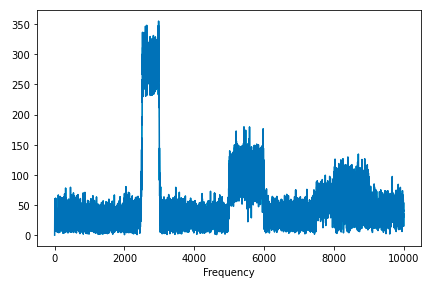
\includegraphics[width=\textwidth]{img/saw_noisy.png}
            \caption{Aliasing effect}
            \label{fig:als_sqr}
        \end{figure}
        
        \begin{figure}[H]
            \centering
            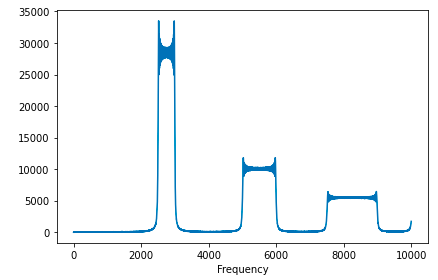
\includegraphics[width=\textwidth]{img/saw_clr.png}
            \caption{Aliasing effect comparison}
            \label{fig:als_clr}
        \end{figure}
            
        By listening them, we can clearly notice the differenct: aliased signal is more "dirty" and "noisy".
            
    \newpage
        \section{Part 4: Glissando}
        
            In this part we need to explore glissando - transition between 2 frequencies. As it was in the Lab1, Halzion track was used.
            
            I've selected a vowel "a" transition segment on 73 second of the record.D
            
            Code of this part - Listing \ref{lst:part4}
            
            \begin{lstlisting}[language=Python,caption=HS operations,label={lst:part4}]
    wave = read_wave('sound/halzion.wav')
    segment = wave.segment(start=73.5, duration=1.5)
    #segment.plot()
    spec = segment.make_spectrum()
    spec.plot(high = 5000)
    segment.make_spectrogram(1024).plot(high=5000)
    decorate(xlabel='Time (s)', ylabel='Frequency (Hz)')
            \end{lstlisting}
            
            Spectrum of the signal looks fine (Figure \ref{fig:part4}), as well as spectrogram does (Figure \ref{fig:part42}. We can clearly see transition of the pitch.
            
            \begin{figure}[H]
                \centering
                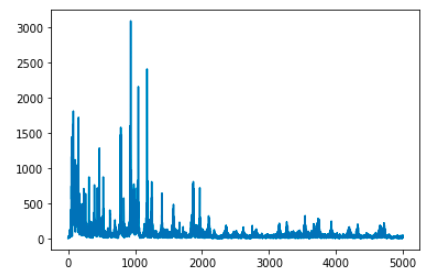
\includegraphics[width=\textwidth]{img/yoasobi_spec.png}
                \caption{Spectrum of a segment}
                \label{fig:part42}
            \end{figure}
            
            \begin{figure}[H]
                \centering
                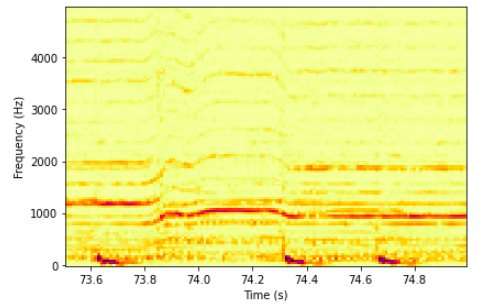
\includegraphics[width=\textwidth]{img/yoasobi_spec2.png}
                \caption{Spectrogram of the segment}
                \label{fig:part42}
            \end{figure}
            
    \newpage
        \section{Part 5: TromboneGliss}
        
            In this part we need to create a class, that provides trombone behavior. It should provide evaluate function, that behaves like trombone would behave by sliding its tube.
            
            Code of the class - Listing \ref{lst:part5_1}
            
            \begin{lstlisting}[language=Python,caption=Definition of the class,label={lst:part5_1}]
    class TromboneGliss(Chirp):
        def evaluate(self, ts):
            l1, l2 = 1.0 / self.start, 1.0 / self.end
            lengths = np.linspace(l1, l2, len(ts) - 1)
            freqs = 1 / lengths
            
            dts = np.diff(ts)
            dphis = PI2 * freqs * dts
            phases = np.cumsum(dphis)
            ys = self.amp * np.cos(phases)
            return ys
            \end{lstlisting}
            
            Code of plotting: Listing \ref{lst:part5_2}.
            
            \begin{lstlisting}[language=Python,caption=Class usage,label={lst:part5_2}]
    wave1 = MyTromboneGliss(262, 349).make_wave(duration=1)
    wave2 = MyTromboneGliss(349, 262).make_wave(duration=1)
    wave1.apodize(); wave2.apodize()
    wave = wave1 | wave2
    wave.make_spectrogram(1024).plot(high=600)
    decorate(xlabel='Time (s)', ylabel='Frequency (Hz)')
    wave.make_audio()
            \end{lstlisting}
            
            As we can see, spectrogram is correct and it looks like exponential one.
            
            \begin{figure}[H]
                \centering
                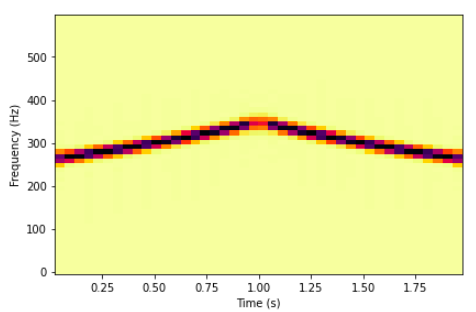
\includegraphics[width=\textwidth]{img/tromb.png}
                \caption{Trombone's spectrogram}
                \label{fig:part5_1}
            \end{figure}
            
    \newpage
        \section{Part 6: Vowels analyze}
        
            In this part we need to make an analysis of vowels. To do it, I used Japanese vowels A I U E O - all their vowels.
            
            Code of spectrogram plotting can be observed on the Listing \ref{lst:aiueo}.
            
                        \begin{lstlisting}[language=Python,caption=Signal and spectrum creation,label={lst:aiueo}]
    wave = read_wave('sound/aiueo.wav')
    segment = wave.segment(start=0, duration=6)
    segment.make_spectrogram(3000).plot(high=1500)
    decorate(xlabel='Time (s)', ylabel='Frequency (Hz)')
            \end{lstlisting}
            
            As we can see on the Figure \ref{fig:part6_1}, Japanese vowels are differs a lot an we can easily say what the sound it is by looking on the spectrogram.
            
            
            \begin{figure}[H]
                \centering
                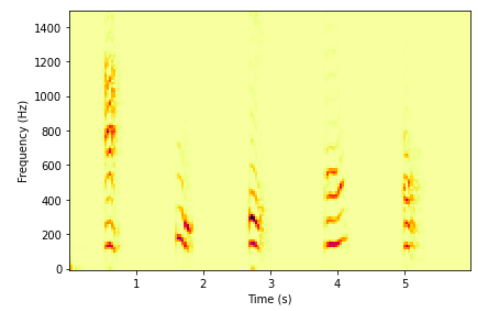
\includegraphics[width=\textwidth]{img/aiueo.png}
                \caption{Spectrum of the signal}
                \label{fig:part6_1}
            \end{figure}
    
    \newpage
        \section{Conclusion}
            More advanced skills and knowledge of signals, waves spectrum and spectrogram was acquired. Spectrum is a good way to visualize a periodic signal, but we cannot use it for the non-periodic signals. But we can split the non-periodic signal into the set of small segments, which we can considered to be a periodic signals (just like it is done with integrals). That allows us to create spectrogram - a set of spectrums at any of the sound. However, we cannot achieve a good time resolution and a good frequency resolution on the same time.
    
\end{document}
